\documentclass[12pt,a4paper,titlepage,twoside]{book}
\usepackage[utf8]{inputenc}
\usepackage[spanish, es-lcroman]{babel}
\usepackage{amsmath}
\usepackage{amsthm}
\usepackage{amsfonts}
\usepackage{amssymb}
\usepackage{graphicx}
\usepackage{lettrine}
\usepackage{float}
\usepackage{color}
\usepackage[top=2cm,bottom=4cm,outer=1.5cm,inner=3cm]{geometry}
\usepackage[nottoc]{tocbibind}	%Para mostrar la bibliografia en el índice
\usepackage{tikz}
\usepackage[refpages]{gloss} % Para el glosario
\usepackage{emptypage} % Para eliminar encabezado de las páginas en blanco
\usepackage{chngcntr}
\usepackage{etoolbox}



% Aquí van algunos comandos para no hacer demasiado largo el preámbulo.


% Separa la lista de figuras por partes
% % % % % % % % % % % % % % % % % % % % % % % % % % % % % % % % % % % % % % % %
%
% NOTA IMPORTANTE: Este comando SIEMPRE debe ir antes de la inclusión del paquete hyperref.
%
% % % % % % % % % % % % % % % % % % % % % % % % % % % % % % % % % % % % % % % % 
% Adaptado de:
%http://tex.stackexchange.com/questions/52746/include-chapters-in-list-of-figures-with-titletoc
\makeatletter
\def\thisparttitle{}\def\thispartnumber{}
\newtoggle{noFigs}

\apptocmd{\@part}%
  {\gdef\thisparttitle{#1}\gdef\thispartnumber{\thepart}%
    \global\toggletrue{noFigs}}{}{}

% the figure environment does the job: the first time it is used after a \chapter command, 
% it writes the information of the chapter to the LoF
\AtBeginDocument{%
  \AtBeginEnvironment{figure}{%
    \iftoggle{noFigs}{
      \addtocontents{lof}{\protect\contentsline {chapter}%
        {\protect\numberline {\thispartnumber} {\thisparttitle}}{}{} }
      \global\togglefalse{noFigs}
    }{}
  }%
}

\makeatother

% Reinicia el contador a 1 en cada parte
\makeatletter
\@addtoreset{chapter}{part} 
\makeatother

% % % % % % % % % % % % % % % % % % % % % % % % % % % % % % % % % % % % % % % % 
\usepackage[colorlinks=true,linkcolor=black,urlcolor=black,citecolor=black]{hyperref}
% % % % % % % % % % % % % % % % % % % % % % % % % % % % % % % % % % % % % % % % 

\counterwithout{figure}{part}

\setlength\parindent{0pt} % Quita la indentación

\renewcommand{\glossname}{Glosario} 

\newtheorem{teorema}{Teorema}

\makegloss

\newcommand*{\autores}{
\begin{tabular}{r l}
GII+GIS: & Jesús Alcalde Alcázar \\
		 & Germán Alonso Azcutia \\
		 & Adrián Gutiérrez Jiménez \\
GIS+MAT: & José Ignacio Escribano Pablos \\
GIS:  	 & Carlos Vázquez Sánchez
\end{tabular}
}

% Incluye archivo para utilizar el comando \portada
%*******************************************************
%                 NO MODIFICAR
\newcommand*{\FSfont}[1]{%
  \fontencoding{T1}\fontfamily{#1}\selectfont}

\newlength{\tpheight}\setlength{\tpheight}{0.9\textheight}
\newlength{\txtheight}\setlength{\txtheight}{0.9\tpheight}
\newlength{\tpwidth}\setlength{\tpwidth}{0.9\textwidth}
\newlength{\txtwidth}\setlength{\txtwidth}{0.9\tpwidth}
\newlength{\drop}
%*******************************************************

% Crea una portada con los siguientes parámetros
%
% #1 : Título 
% #2 : Subtítulo
% #3 : Subsubtítulo
% #4 : Autor(es)
% #5 : Lugar
%

\newcommand*{\portada}[5]{
\begin{titlepage}
\begingroup
\vspace*{1cm}
\drop = 0.2\txtheight
\centering
\vfill
{\Huge \scshape #1}\\[\baselineskip]
{\Large \textbf{#2}}\\[\baselineskip]
{\Large \scshape #3}\\[\baselineskip]
\vspace*{0.3cm}
{\large \textit{#4}}\\[0.5\drop]

\includegraphics[scale=0.35]{./images/logoURJC.jpg}
\vspace*{1.5cm}

{\large \scshape #5, \today} \par
\begin{center}
\end{center}
\vfill\null
\endgroup
\end{titlepage}
}
 %*****************************************************
 

\usepackage{tikz}
\usepackage{xstring}

% Aquí van todas las figuras en TikZ, hay que asignarlas un numero para poder cambiar todas a la vez.

\newcommand{\figura}[1]{
	\IfEqCase{#1}{
	% PARTE I %
		{hipervisor1}{\figurahipA}
		{hipervisor2}{\figurahipB}
		{hipervisor2real}{\figurahipBfin}
		{hardware}{\figuraHard}
		{sohost1}{\figuraSO}
		{sohost2}{\figuraSOsimpl}
		{hipervisor}{\fbox{\textcolor{red}{ESTA FIGURA HAY QUE HACERLA}}}
		{maqinavirtual}{\fbox{\textcolor{red}{ESTA FIGURA HAY QUE HACERLA}}}
		{virtualizacionnat}{\fbox{\textcolor{red}{ESTA FIGURA HAY QUE HACERLA}}}
		{virtualizacionhost}{\fbox{\textcolor{red}{ESTA FIGURA HAY QUE HACERLA}}}
		{vmware}{\fbox{\parbox{70mm}{\textcolor{red}{ESTA FIGURA HAY QUE HACERLA\\ ES COMO LA ÚLTIMA PERO LAS VM ESTAN EL EL SERVIDOR}}}}
	% PARTE II %
		{3}{\pizarra}
	}[\PackageError{figura}{Figura no declarada: #1}{}]
}


% Aqui se añaden las figuras %
\newcommand{\figurahipA}{
\begin{tikzpicture}
	\draw[rounded corners=3mm, fill=gray!30, thick] (0.05,2) rectangle (1.95,4);
	\draw[rounded corners=3mm, fill=gray!30, thick] (2.05,2) rectangle (3.95,4);
	\draw[rounded corners=3mm, fill=gray!30, thick] (6.05,2) rectangle (7.95,4);
	\draw[rounded corners=3mm, fill=gray!30, thick] (8.05,2) rectangle (9.95,4);
	\draw[rounded corners=3mm, fill={blue!40}, thick] (0,1) rectangle (10,2); 
	\draw[rounded corners=3mm, fill=yellow!40, thick] (0,0) rectangle (10,1); 

	\node at (1,3) {${VM}_1$};
	\node at (3,3) {${VM}_2$};
	\node at (5,3) {\textbf{...}};
	\node at (7,3) {${VM}_{n-1}$};
	\node at (9,3) {${VM}_n$};
	\node at (5,1.5) {\textsc{Hipervisor o VMM}};
	\node at (5,0.5) {\textsc{Hardware}};
\end{tikzpicture}
}

\newcommand{\figurahipB}{
\begin{tikzpicture}
	\draw[rounded corners=3mm, fill=gray!30, thick] (0.05,3) rectangle (1.95,5);
	\draw[rounded corners=3mm, fill=gray!30, thick] (2.05,3) rectangle (3.95,5);
	\draw[rounded corners=3mm, fill=gray!30, thick] (6.05,3) rectangle (7.95,5);
	\draw[rounded corners=3mm, fill=gray!30, thick] (8.05,3) rectangle (9.95,5);
	\draw[rounded corners=3mm, fill={blue!40}, thick] (0,2) rectangle (10,3);
	\draw[rounded corners=3mm, fill={red!40}, thick] (0,1) rectangle (10,2); 
	\draw[rounded corners=3mm, fill=yellow!40, thick] (0,0) rectangle (10,1); 

	\node at (1,4) {${VM}_1$};
	\node at (3,4) {${VM}_2$};
	\node at (5,4) {\textbf{...}};
	\node at (7,4) {${VM}_{n-1}$};
	\node at (9,4) {${VM}_n$};
	\node at (5,2.5) {\textsc{Software de virtualización}};
	\node at (5,1.5) {\textsc{Sistema operativo} {\tiny (Anfitrión)}};
	\node at (5,0.5) {\textsc{Hardware}};
\end{tikzpicture}
}

\newcommand{\figurahipBfin}{
\begin{tikzpicture}
	\draw[rounded corners=3mm, fill=green!30, thick] (0,2) rectangle (1.90,5);
	\draw[rounded corners=3mm, fill=gray!30, thick] (2.05,3) rectangle (3.95,5);
	\draw[rounded corners=3mm, fill=gray!30, thick] (6.05,3) rectangle (7.95,5);
	\draw[rounded corners=3mm, fill=gray!30, thick] (8.05,3) rectangle (9.95,5);
	\draw[rounded corners=3mm, fill={blue!40}, thick] (2,2) rectangle (10,3);
	\draw[rounded corners=3mm, fill={red!40}, thick] (0,1) rectangle (10,2); 
	\draw[rounded corners=3mm, fill=yellow!40, thick] (0,0) rectangle (10,1); 

	\node at (1,4) {Apps};
	\node at (1,3.5) {del};
	\node at (1,3) {S.O};
	\node at (3,4) {${VM}_1$};
	\node at (5,4) {\textbf{...}};
	\node at (7,4) {${VM}_{n-1}$};
	\node at (9,4) {${VM}_n$};
	\node at (6,2.5) {\textsc{Software de virtualización}};
	\node at (5,1.5) {\textsc{Sistema operativo} {\tiny (Anfitrión)}};
	\node at (5,0.5) {\textsc{Hardware}};
\end{tikzpicture}
}

\newcommand{\figuraHard}{
\begin{tikzpicture}
	\draw[rounded corners=3mm, fill=yellow!40, thick] (-0.05,-0.05) rectangle (10.05,3.05);

	\node at (2,2.5) {\textsc{Hardware Real}};
	
	\node at (1.25,1.4) {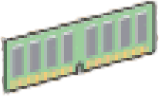
\includegraphics{./images/memoria.png}};
	\node at (1.25,0.5) {\textsc{Memoria}};
	
	\node at (3.75,1.4) {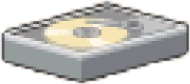
\includegraphics{./images/hdd.png}};
	\node at (3.75,0.5) {\textsc{Disco}};
	
	\node at (6.25,1.4) {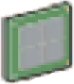
\includegraphics{./images/cpu.png}};
	\node at (6.25,0.5) {\textsc{CPU}};
	
	\node at (8.75,1.4) {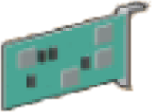
\includegraphics{./images/red.png}};
	\node at (8.75,0.5) {\textsc{Red}};
\end{tikzpicture}
}

\newcommand{\figuraSO}{
\begin{tikzpicture}
\definecolor{morado}{RGB}{177,100,177}
	\draw[rounded corners=3mm, fill=green!30, thick] (-.50,3) rectangle (6.5,4);
	\draw[rounded corners=3mm, fill=red!40, thick] (0,0) rectangle (6,3);
	\draw[rounded corners=3mm, fill=morado!40, thick] (0.5,0) rectangle (5.5,2);
	\draw[rounded corners=3mm, fill=blue!30, thick] (1,0) rectangle (5,1);
	\draw[rounded corners=3mm, fill=yellow!40, thick] (1.5,-1) rectangle (4.5,0);
	
	\node at (3,3.5) {\textsc{Aplicaciones}};
	\node at (2.2,2.5) {\textsc{Sistema Operativo}};
	\node at (2.5,1.5) {\textsc{Apps del SO}};
	\node at (3,0.6) {\textsc{Kernel}};
	\node at (3,-0.5) {\textsc{Hardware}};
\end{tikzpicture}
}

\newcommand{\figuraSOsimpl}{
\begin{tikzpicture}
	\draw[rounded corners=3mm, fill=green!30, thick] (-0.5,1) rectangle (6.5,2);
	\draw[rounded corners=3mm, fill=red!40, thick] (0,0) rectangle (6,1);
	\draw[rounded corners=3mm, fill=yellow!40, thick] (1.5,-1) rectangle (4.5,0);
	
	\node at (3,1.5) {\textsc{Aplicaciones}};
	\node at (3,0.5) {\textsc{Sistema Operativo}};
	\node at (3,-0.5) {\textsc{Hardware}};
\end{tikzpicture}
}


\newcommand{\pizarra}{
\begin{tikzpicture}
	\draw[fill=brown!90] (0,0) rectangle (6,3);
	\draw[fill=green!40] (0.2, 0.2) rectangle (5.8,2.8);
	
	\draw[fill=red!40] (7.5,2.25) ellipse (1cm and 0.5cm);
	\draw[fill=blue!40] (7.5,0.75) ellipse (1cm and 0.5cm);
	\draw[fill=yellow!40] (1.5,-1.5) ellipse (0.5cm and 1cm);
	\draw[fill=purple!50] (4.5,-1.5) ellipse (0.5cm and 1cm);
	\draw[fill=gray!30] (-1.5,0.75) ellipse (1cm and 0.5cm);
	\draw[fill=white!40] (-1.5,2.25) ellipse (1cm and 0.5cm);
	\draw[fill=orange!40] (1.5,4.5) ellipse (0.5cm and 1cm);
	\draw[fill=pink!40] (4.5,4.5) ellipse (0.5cm and 1cm);
	
	\draw[<->] (6,0.75) -- (6.5,0.75);
	\draw[<->] (6,2.25) -- (6.5,2.25);
	\draw[<->] (1.5,3) -- (1.5,3.5);
	\draw[<->] (4.5,3) -- (4.5,3.5);
	\draw[<->] (0,0.75) -- (-0.5,0.75);
	\draw[<->] (0,2.25) -- (-0.5,2.25);
	\draw[<->] (1.5,-0.5) -- (1.5,0);
	\draw[<->] (4.5,-0.5) -- (4.5,0);
	
	\node at (3,1.5) {\textsc{Pizarra}};
	\node at (7.5,2.25) {\textsc{Agente}};
	\node at (7.5,0.75) {\textsc{Agente}};
	\node[rotate=90] at (1.5,-1.5) {\textsc{Agente}};
	\node[rotate=90] at (4.5,-1.5) {\textsc{Agente}};
	\node at (-1.5,0.75) {\textsc{Agente}};
	\node at (-1.5,2.25) {\textsc{Agente}};
	\node[rotate=90] at (1.5,4.5) {\textsc{Agente}};
	\node[rotate=90] at (4.5,4.5) {\textsc{Agente}};
\end{tikzpicture}
}


% Reinicia el contador a 1 en cada parte
\makeatletter
\@addtoreset{chapter}{part} 
\makeatother

\begin{document}

\frontmatter % Incluye índice, portada, prefacio, ...
 
% Portada
\portada{Práctica Obligatoria}{Diseño y Arquitectura del Software}{\ }{\autores}{Móstoles}
% Fin Portada

\tableofcontents
%\thispagestyle{empty}


\chapter*{Prefacio}
\addcontentsline{toc}{chapter}{Prefacio}
\lettrine[lines=1,slope=4pt,findent=0pt]{E}{}sto es un prefacio.\\

\section*{Objetivos y motivaciones}
Tanto en el ámbito informático académico como en el profesional, en ocasiones puede ser necesario un cambio de sistema operativo a la hora de trabajar. Esto puede estar ocasionado tanto por requisitos del lenguaje a utilizar, por una arquitectura más adecuada o simplemente por cuestión de preferencias. Pero estos cambios implicarían una CPU para cada sistema operativo, lo que lo haría terriblemente ineficiente desde el punto de vista económico, ergonómico y logístico. \\
Por ello es necesario conocer la arquitectura del software que permita escoger entre más de un sistema operativo, y que el adicional (aún sin llegar al nivel de eficiencia del sistema nativo) trabaje a un nivel óptimo.\\
Pero además de observar y comprender la arquitectura de un software conocido y utilizado comercialmente, también son necesarios los conocimientos necesarios para poder diseñar a un nivel de arquitectura y diseño el funcionamiento de una plataforma. Para ello crearemos una biblioteca en la que cualquier usuario podrá programar un agente capaz de leer y escribir en una pizarra potencialmente remota.\\
Por tanto los dos principales objetivos de la práctica serán:
\begin{itemize}
\item Definir la arquitectura de un sistema de virtualización.
\item Describir la arquitectura y diseño de una plataforma que implemente la arquitectura de pizarra que pueda ser utilizada por otros programas.
\end{itemize}

\section*{Estructura de la memoria}
Debido a las dos partes claramente diferenciadas e la práctica, se harán dos secciones claramente diferenciadas :
\begin{itemize}
\item Parte de OBSERVACIÓN: en la que tras una pequeña introducción se detallará la arquitectura del sistema escogido
\item Parte de DISEÑO: \textcolor{red}{UNA VEZ ACABADOS LOS REQUISITOS, UML Y DEMÁS ACTUALIZAR ESTA SECCIÓN}
\end{itemize}

\section*{GitHub}
Para la realización de esta práctica hemos utilizado el software \textbf{GitHub}, propiedad de 	{GitHub Inc}, el cual nos ha permitido trabajar sobre un repositorio al que todos los miembros del grupo teníamos acceso. Hemos elegido usar GitHub por los siguientes motivos:
\begin{itemize}
	\item Es un conocido programa para desarrolladores de software, lo que nos ha permitido trabajar de una forma profesional.
	\item Al ser un alto número los integrantes del grupo, nos ha sido más fácil y sencillo trabajar mediante repositorios. 
	\item Pero principalmente debido a que dicho programa sigue una arquitectura de pizarra y soporta el conocido framework ``Ruby on Rails", lo que nos acercaba a un entorno práctico a los dos aspectos a tratar en la práctica: los framework y la arquitectura de pizarra.
\end{itemize}

\color{red}
FALTA:
\begin{itemize}
%\item Explicar la forma de trabajo \textit{(De forma distribuida mediante GitHub)}
\item Si se hace código, recalcarlo mucho.
\item Dar paso al inicio de la primera parte.
\end{itemize}
\color{black}



\chapter*{Nota}
\addcontentsline{toc}{chapter}{Nota}
\chapter [GitHub]{Nota}
Para la realización de esta práctica hemos utilizado el software {\bf GitHub}, propiedad de 	GitHub Inc, el cual nos ha permitido trabajar sobre un repositorio al que todos los miembros del grupo teníamos acceso. Hemos elegido usar GitHub por los siguientes motivos:
\begin{itemize}
	\item Es un conocido programa para desarrolladores de software, lo que nos ha permitido trabajar de una forma profesional
	\item Al ser un alto número los integrantes del grupo, nos ha sido más fácil y sencillo trabajar mediante repositorios, 
	\item Pero principalmente debido a que dicho programa sigue una arquitectura de pizarra y soporta el conocido framework 'Ruby on Rails', lo que nos acercaba a un entorno práctico a los dos aspectos a tratar en la práctica: los framework y la arquitectura de pizarra.
\end{itemize}


\mainmatter % Parte principal

\part{Observación}
\chapter{Introducción}
\lettrine[lines=1,slope=4pt,findent=0pt]{E}{}n esta primera parte de la memoria nos vamos a encargar de hacer una descripción a nivel arquitectónico de los sistemas de virtualización de las aulas de la Universidad Rey Juan Carlos.\\

\noindent Como nos vamos a centrar en los ordenadores de las aulas, éstos se encuentran virtualizados con VMware~\cite{vmware}



\part{Diseño}
\chapter{Introducción}
\lettrine[lines=1,slope=4pt,findent=0pt]{E}{}n esta primera parte de la memoria nos vamos a encargar de hacer una descripción a nivel arquitectónico de los sistemas de virtualización de las aulas de la Universidad Rey Juan Carlos.\\

\noindent Para llevar a cabo esta tarea hemos decidido que la mejor opción pasa por describir o analizar qué es un sistema de virtualización, para después poder centrarnos en el caso concreto de las aulas de la URJC, que se encuentran virtualizadas con VMware\cite{vmware} lo que significa que en el caso concreto nos centraremos en VMware, eso sí, haciendo continuas analogías a lo que se ve en las aulas.\\

\noindent Pero para entrar un poco en materia vamos a intentar explicar brevemente qué es esto de la \emph{virtualización}.

\section{¿Qué es la virtualización?}
\noindent Con la intención de hacernos una idea precisa de \emph{virtualización} hemos buscado diversas definiciones, de las cuales nos quedamos con:
\begin{quote}
\emph{<<Virtualización es la creación -a través de software- de una versión virtual de algún recurso tecnológico, como puede ser una plataforma de hardware, un sistema operativo, un dispositivo de almacenamiento u otros recursos de red.>>}
\begin{flushright}
--Wikipedia\cite{defvirwiki}
\end{flushright}
\end{quote}

\noindent Es otras palabras, la creación mediante software de elementos hardware virtuales. Un buen ejemplo de ésto es cuando particionamos un disco duro; físicamente tenemos un HDD pero a nivel de software existen dos, pues el disco duro esta \emph{virtualizado} en dos particiones.\\

\noindent Dando una vuelta de tuerca más, podemos definir \emph{virtualización} como el proceso por el cual una capa de software(VMM o \emph{Virtual Machine Monitor}) abstrae los recursos de la computadora física al Sistema Operativo o \emph{Máquina Virtual}.

\section{¿Qué es una máquina virtual?}

\noindent Al igual que antes, encontramos diversas acepciones de \emph{máquina virtual}, pero vamos a partir de la definición de \emph{Wikipedia} pues es la más completa.

\begin{quote}
\emph{<<Una máquina virtual es un software que simula a una computadora y puede ejecutar programas como si fuese una computadora real. Este software en un principio fue definido como \textquotedblleft un duplicado eficiente y aislado de una máquina física\textquotedblright.>>}
\begin{flushright}
--Wikipedia\cite{defmaqvirwiki}
\end{flushright}
\end{quote}

\noindent Podemos encontrar dos tipos de éstas:

\begin{itemize}
\item \textbf{Máquinas virtuales de proceso} o máquina virtual de aplicación, se ejecuta como un proceso normal dentro de un sistema operativo y soporta un solo proceso. Su objetivo es el de proporcionar un entorno de ejecución independiente del sistema operativo y del hardware. Una máquina virtual de proceso muy popular es la de Java(\emph{Java Virtual Machine}).
\item \textbf{Máquinas virtuales de sistema} o máquinas virtuales de hardware, que permiten a la máquina física multiplicarse entre varias máquinas virtuales, cada una con su propio sistema operativo. A la capa de software que se permite la virtualización se la llama \emph{monitor de máquina virtual} o \emph{Virtual Machine Monitor}, anteriormente mencionado.
\end{itemize}

\noindent Como es obvio nosotros nos vamos a centrar en la última.

\section{Condiciones para la virtualización}

\noindent Para llevar a cabo una virtualización del sistema, Popek y Goldberg escribieron en un artículo\cite{reqvir} qué condiciones se han de dar para una virtualización eficiente, para ello dividieron el repertorio de instrucciones en:
\begin{itemize}
\item \textbf{Instrucciones privilegiadas:} Las que sólo funcionan en modo kernel y no en modo usuario.
\item \textbf{Instrucciones sensibles de control:} Las que cambian la configuración del sistema.
\item \textbf{Instrucciones sensibles de comportamiento:} Aquellas que dependen de la configuración de los recursos. 
\end{itemize}

\noindent Y como resultado de su análisis formularon estos teoremas.
\begin{teorema}
Para cualquier computadora convencional de tercera generación, se puede construir un VMM efectivo si el conjunto de instrucciones sensibles es un subconjunto de las instrucciones privilegiadas.
\end{teorema}
\begin{teorema}
Una máquina convencional de tercera generación es recursivamente virtualizable si es virtualizable y se puede construir para ella un VMM sin ninguna dependencia de sincronización.
\end{teorema}
\noindent Con esto volveremos más adelante, ahora centrémonos en su arquitectura.
\chapter[Descripción de la arquitectura]{Descripción de la arquitectura de virtualización}

\lettrine[lines=1,slope=4pt,findent=0pt]{U}{}na vez introducido el vocabulario básico y tras haber indagado un poco más en la materia vamos a centrarnos en la arquitectura como tal.\\

\section{Tipos de Virtualización}\label{tiposvir}
En el apartado anterior ya se pudo vislumbrar que existen diferentes formas de virtualización, y por ello, vamos a hacer un pequeño análisis de cada uno, pero antes nos interesa conocer el término \emph{\gloss{HYP}}, ya que es el elemento central de un sistema de máquinas virtuales.

\subsection{¿Qué es un hipervisor?}
El \emph{\gloss{HYP}} o \emph{\gloss[long]{VMM}} se trata de una plataforma que permite aplicar diversas técnicas de control para utilizar, al mismo tiempo, diferentes sistemas operativos en una misma computadora.\\

Se trata de un elemento software que dependiendo de cómo se sitúe en relación con el Hardware da lugar a dos maneras diferentes de virtualizar, dos tipos de \emph{\gloss{HYP}}\cite{tipoship}:

\subsection{Hipervisor de Tipo 1 o \emph{Nativo}}\label{tiposvir1}
 El software del hipervisor se ubica directamente entre el hardware y las distintas máquinas virtuales, para ofrecer la funcionalidad descrita, siguiendo la siguiente estructuración:

\begin{figure}[H]
\begin{center}
\figura{hipervisor1}
\end{center}
\caption[Hipervisor Tipo 1]{Esquema de un hipervisor de primer nivel}
\end{figure}

Este tipo de \emph{hipervisor} también es conocido como \emph{unhosted} o \emph{bare metal}, que en inglés hacen referencia a que no es huésped o que se ejecuta a bajo nivel, respectivamente.\\

Dentro de este tipo se encuentran VMware ESXi, VMware ESX y Microsoft Hyper-V Server, pero nos gustaría presta una atención especial a \gloss{XEN} por ser un hipervisor de código abierto desarrollado por la Universidad de Cambridge\cite{proyectoxen}\cite{proyectoxen2}.
\subsection{Hipervisor de Tipo 2 o \emph{Huésped}}\label{tiposvir2}
Es una arquitectura alternativa para la máquina virtual insertando una capa de virtualización encima del sistema operativo \emph{host} o huésped, siendo éste responsable de administrar el hardware. Los sistemas operativos invitados se instalarán encima del nivel de virtualización, en máquinas virtuales. Tiene la siguiente estructura:

\begin{figure}[H]
\begin{center}
\figura{hipervisor2}
\end{center}
\caption[Hipervisor Tipo 2]{Esquema de un hipervisor de segundo nivel}
\end{figure}

Este tipo de hipervisor tiene una ventaja muy destacada, el usuario puede instalar esta arquitectura de máquina virtual sin modificar el sistema operativo host pudiendo descansar en el sistema operativo host para entregar los controladores de dispositivos y otros servicios de bajo nivel (se simplifica el diseño de la máquina virtual y facilita la implementación).\\

Otra característica suya es que al ejecutarse sobre un sistema operativo huésped, éste puede ejecutar sus propias aplicaciones, por lo que en realidad el esquema completo sería:

\begin{figure}[H]
\begin{center}
\figura{hipervisor2real}
\end{center}
\caption[Hipervisor Tipo 2 final]{Esquema de un hipervisor de segundo nivel real}
\end{figure}

Algunos de los hipervisores tipo 2 más utilizados son: Oracle: VirtualBox, VirtualBox OSE, VMware: Workstation; siendo éste último en el que más nos vamos a centrar.

\section{Componentes}
En las figuras mostradas anteriormente, se han hecho referencias a \emph{hardware}, \emph{\gloss{{HYP}}} o \emph{\gloss[long]{MAQVIR}} en las que no explicamos exactamente que significa y por ello, ahora, vamos a analizar cada uno de estas partes descomponiendo sus componentes; es decir, qué elementos lo forman, para después poder juntarlos todos y obtener una idea real de la arquitectura.\\

Vamos a seguir un órden, de menor a mayor nivel, comenzaremos con el \emph{hardware} para terminar con las distintas \emph{VMs}.

\subsection{Hardware o Hardware real}
Quizás lo primero que tengamos que hacer es explicar el encabezado del apartado, ¿Por qué \emph{\textquotedblleft harware real\textquotedblright}.\\
Para contestar a esto es necesario conocer los componentes de una máquina virtual (\textit{Véase apartado \ref{apartadomaqvir}}), pues esta tiene también elementos hardware y el calificativo \emph{\textquotedblleft real\textquotedblright} es lo que los diferencia.\\

Este elemento hardware se refiere, como es obvio, al computador físicamente hablando, es decir, al aparato electrónico generalmente conectado a una toma de luz y sus componentes físicos: l memoria RAM, el \gloss[short]{HDD}  y su \gloss[short]{CPU}. Por tanto, a partir de ahora vamos a representar el hardware como:

\begin{figure}[H]
\begin{center}
\figura{hardware}
\end{center}
\caption[Hardware Real]{Esquema del hardware real}
\end{figure}

\subsection{Sistema Operativo huésped}\label{sohost}
En este caso no se trata nada más que de un simple sistema operativo y lo que esto conlleva, su funcionalidad y sus restricciones.\\

Cualquier sistema operativo se puede descomponer en los archivos del sistema o \emph{\gloss{KERNEL}} y de las aplicaciones que se ejecutan sobre este sistema, es decir que el esquema es el siguiente:

\begin{figure}[H]
\begin{center}
\figura{sohost1}
\end{center}
\caption[Sistema Operativo huésped]{Esquema de componentes de un Sistema Operativo \emph{host} o huésped}
\end{figure}

Cabe destacar que se trata de una manera un poco redundante, tal y cómo estaba representado antes el sistema operativo nos bastaba, y por ello nos vamos a quedar con esta representación:

\begin{figure}[H]
\begin{center}
\figura{sohost2}
\end{center}
\caption[Sistema Operativo huésped simplificado]{Esquema de componentes de un Sistema Operativo \emph{host} o huésped de manera simplificada}
\end{figure}

\subsection{Hipervisor}
Ahora nos centramos en el meollo de asunto, pero,en realidad,¿nos es relevante el contenido del \gloss{HYP} o \gloss[long]{VMM}?\\

Para lo que nosotros vamos a profundizar y a lo que queremos llegar, nos es completamente irrelevante, pero como nunca esta de más conocer cosas nuevas simplemente vamos a decir los componentes de un hipervisor varían según el \emph{\textquotedblleft fabricante\textquotedblright} y el tipo.\\

Aun así, existen una serie de elementos comunes para todos ellos, son los referentes a la organización del sistema virtual, por lo que podemos concluir con la siguiente figura:

\begin{figure}[H]
\begin{center}
\figura{hipervisor}
\end{center}
\caption[Componentes hipervisor]{Esquema de componentes del hipervisor}
\end{figure}

Aquí, al igual que en el caso del sistema operativo (\textit{Véase apartado \ref{sohost}}) utilizaremos el esquema que ya teníamos en lugar de éste a partir de ahora.

\subsection{Máquina Virtual}\label{apartadomaqvir}
Sin necesidad de pensar mucho, y con la comparativa de que una máquina virtual simula el comportamiento de un computador real, es fácil pensar que ésta se compone de manera similar a un computador y acertaríamos, este es su esquema:

\begin{figure}[H]
\begin{center}
\figura{maqinavirtual}
\end{center}
\caption[Maquina Virtual]{Esquema de componentes de una máquina virtual}
\end{figure}

Si seguimos la lógica de capas y abstracción, el encapsulamiento que se produce entre el \emph{harware virtual} y el sistema operativo, hacen que éste último no diferencie sobre qué se esta ejecutando. Esto es un punto importante en los sistemas de virtualización, ya que gracias a esto no es necesario adaptar el software a poder ser ejecutado en máquinas virtuales, tan sólo necesitamos instalar un \gloss{HYP}.


\section{Esquema general}
Puestos a hacer un resumen, vamos a agrupar todos los elementos que participan en los sistemas de virtualización con sus correspondientes componentes en una única representación.\\

Como esta representación varía dependiendo del tipo de virtualización que escojamos, vamos a realizar una representación para cada uno.

\subsection{Virtualización \emph{nativa}}
Para todos los sistemas de virtualización que utilizan un hipervisor de tipo 1 como elemento central, esta es su arquitectura:

\begin{figure}[H]
\begin{center}
\figura{virtualizacionnat}
\end{center}
\caption[Virtualización \emph{nativa}]{Esquema general de un sistema de virtualización de primer nivel}
\end{figure}

\subsection{Virtualización \emph{host}}
Para todos los sistemas de virtualización que utilizan un hipervisor de tipo 2 como elemento virtualizador, esta es su arquitectura:

\begin{figure}[H]
\begin{center}
\figura{virtualizacionhost}
\end{center}
\caption[Virtualización \emph{host}]{Esquema general de un sistema de virtualización de segundo nivel}
\end{figure}

\backmatter % Bibliografia, lista de figuras, glosario, ...
\newpage{\ } %Añadida página para que no acabe y comience el glosario

\printgloss{./glosario}

\listoffigures

\bibliographystyle{plain}
\bibliography{./bibliografia/bibliografia}



\end{document}
